\chapter{Introduciton}
Briefly describe the science or engineering problem to be addressed in the report, as well as the purpose and usefulness of the device or system you have built. Summarize the contents of the upcoming chapters as well as the main conclusions of your project, to be elaborated in the last chapter.

\section{Section head}
To create a section head, type \verb|\section{}| and put the section name into the brackets. It automatically formats as above and creates a table of contents entry (after you compile the project twice using Xe\TeX or Lua\TeX, or once using latexmk). \TeX will not make the capitalization consistent; you have to do that yourself.

Figure 1 is an example of figure and caption style. Table 1 is an example of table and table title style. A starter table for parts costs is in Chapter 4 of this template.

\begin{figure}[H]
    \centering
    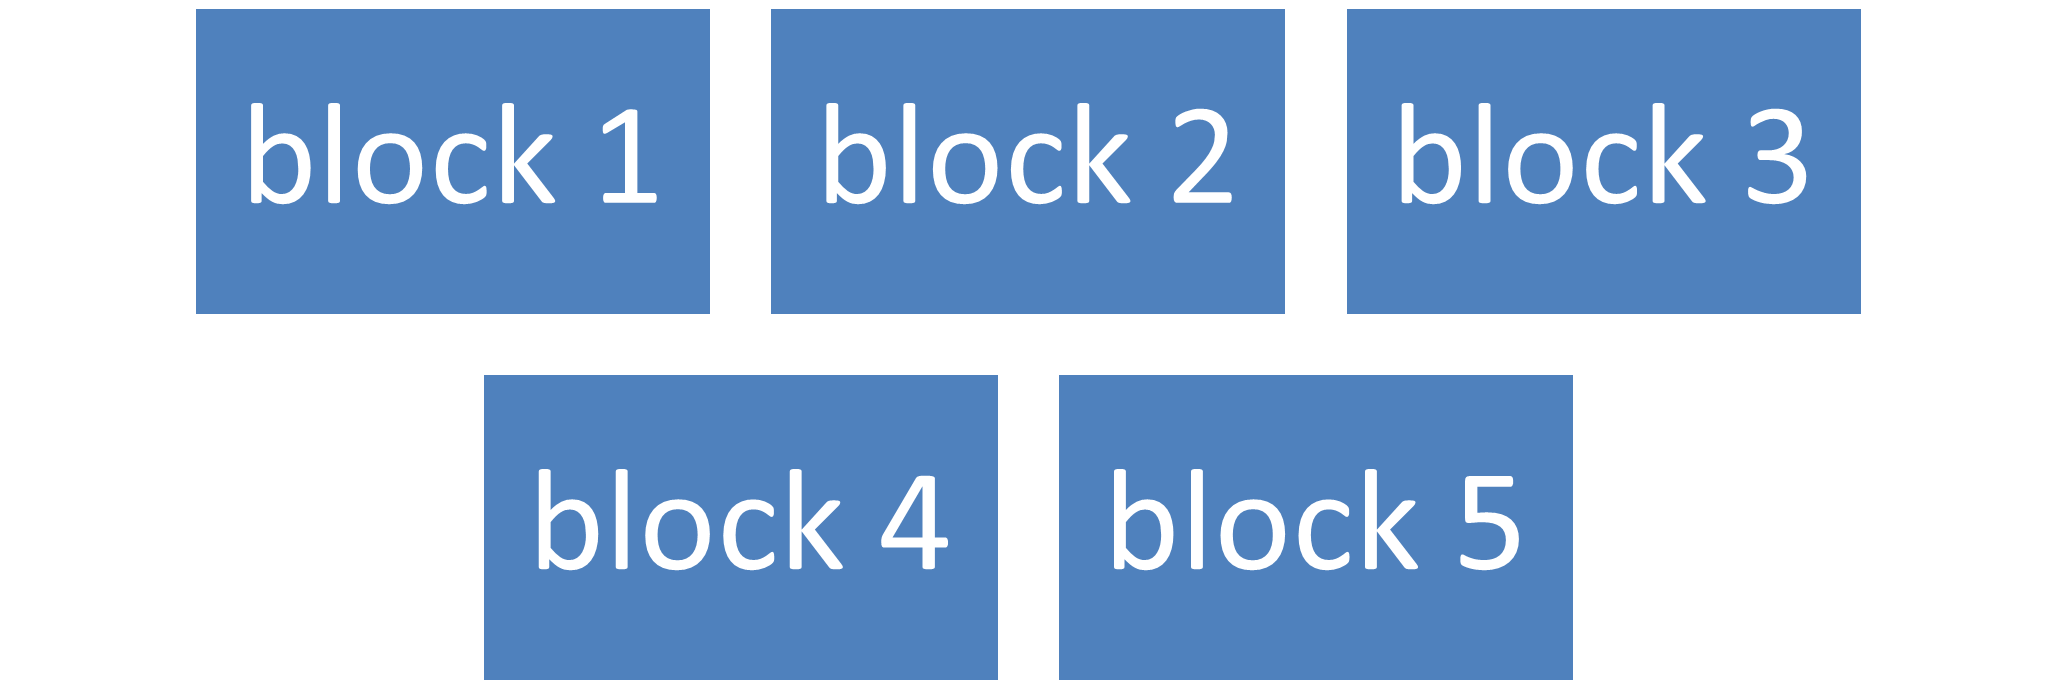
\includegraphics[width=\textwidth]{figs/Picture1.png}
    \caption{Example of placement and caption for a block diagram. Size the figure so that one-inch margins are preserved. Group the figure and caption to hold them together.}
\end{figure}
\begin{table}[H]
    \centering
    \caption{Example of a Table and Its Title}
    \begin{tabular}{@{}ccc@{}}
    \toprule
    \bf Part & \bf Electricity & \bf Magnetism \\ \midrule
    Field intensity & $\mathbf{E}$ & $\mathbf{H}$ \\
    Flux density & $\mathbf{D}$ & $\mathbf{B}$ \\
    Constitutive factor & $\epsilon^b$ & $\mu^c$ \\ \bottomrule
    \end{tabular}
\end{table}